\documentclass[titlepage]{article}
\usepackage[a4paper,includehead,includefoot,headheight=10pt,headsep=2mm,width=17cm,height=27cm,footskip=0.5cm]{geometry}
\usepackage{cmap}
%\usepackage{hyperref}
\usepackage[T1]{fontenc}
\usepackage[utf8]{inputenc}
\usepackage[russian]{babel}
\usepackage{graphicx}
\usepackage{xcolor}
\usepackage{amssymb}
\usepackage{amsmath}
\usepackage{physics}
\usepackage{wrapfig}
\usepackage{pdfpages}

\usepackage{pgfplots}
\pgfplotsset{width=7cm,compat=newest}

\usepackage{amsmath}
\DeclareMathOperator\arctanh{arctanh}

\usepackage{amsmath}
\DeclareMathOperator\arccosh{arccosh}

\usepackage{amsmath}
\DeclareMathOperator\const{const}

\begin{document}
\section{Как далеко видно с горы}

\subsection{Формулировка задачи}
Рассмотрим следующую задачу. Как далеко может видеть наблюдатель, находящийся на вершине горы высоты $h$? Землю считать шарообразной, влиянием воздуха пренебречь. 

\subsection{Строгое решение задачи}
Во\--первых, ясно, что конечность дальности обзора связанна с кривизной поверхности Земли, если бы планета была плоской, то в отсутствии воздуха ничто бы не препятствовало наблюдению сколь угодно далёких мест на её поверхности. Если наблюдатель смотрит в данном направлении, то его взор охватывает лишь ту часть поверхности Земли, что расположена ниже касательной, проведённой из глаз наблюдателя к поверхности Земли. Точка касания соответствует точке на горизонте. 

\par
Во\--вторых, так как в рамках рассматриваемой задачи форма Земли полагается шарообразной, то становится не важным направление, в котором смотрит наблюдатель. В какую бы сторону он не посмотрел~\----~вид будет тот же самый. Поэтому можно рассматривать лишь сечение системы наблюдатель\--Земля плоскостью, проходящей через центр Земли и касательную, соединяющую глаза наблюдателя с точкой на горизонте. Получаем обычную школьную геометрическую задачу.
\begin{figure}[h]
 \centering
 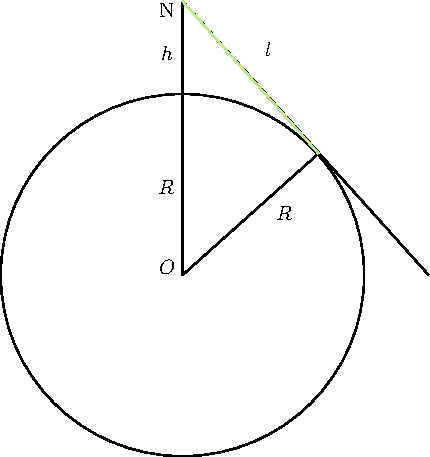
\includegraphics[scale = 0.8]{first1.pdf}
 \caption{Чертёж к задаче о дальности обзора}
 \label{fig:1}
\end{figure}
\par
Нужно найти расстояние $l$ (см. рис. \ref{fig:1}). Для этого воспользуемся теоремой Пифагора. Касательная, радиус Земли и отрезок, соединяющий наблюдателя с центром Земли, образуют прямоугольный треугольник, для сторон которого справедливо:
\begin{equation}
 (R+h)^2 = R^2 + l^2
\end{equation}
Из данного выражения нетрудно получить искомое расстояние:
\begin{equation}\label{eq:1}
 l = \sqrt{2Rh + h^2}
\end{equation}

\subsection{Упрощение ответа}
Полученный результат может быть труден для запоминания. Зададимся вопросом о таком упрощении данной формулы, которое будет крайне слабо отражаться на ответе.

\par
Оценим входящие в формулу (\ref{eq:1}) величины. Радиус Земли $R$ равен примерно $6 370$ км, в то время как высота горы $h$ не может быть больше $9$ км. Тогда выходит, что первое подкоренное слагаемое порядка десятков тысяч квадратных километров, а второе порядка десятков квадратных километров. Разумно пренебречь вторым слагаемым, ведь оно крайне слабо влияет на ответ. Оно даёт ошибку только в четвёртом знаке, что зачастую не важно. Таким образом приходим к более простой формуле:
\begin{equation}
 l = \sqrt{2Rh}
\end{equation}

Проиллюстрируем графиком (см. рис. \ref{fig:2}) тот факт, что используемое приближение и вправду не сильно меняет ответ. Видно, что точный и приближенный результаты почти не различимы. Если рассматривать зависимость от $h$, то видно, что она не линейная, а корневая, то есть если подняться в сто раз выше, то видно станет лишь в десять раз дальше.

\begin{figure}[htb]
 \centering
 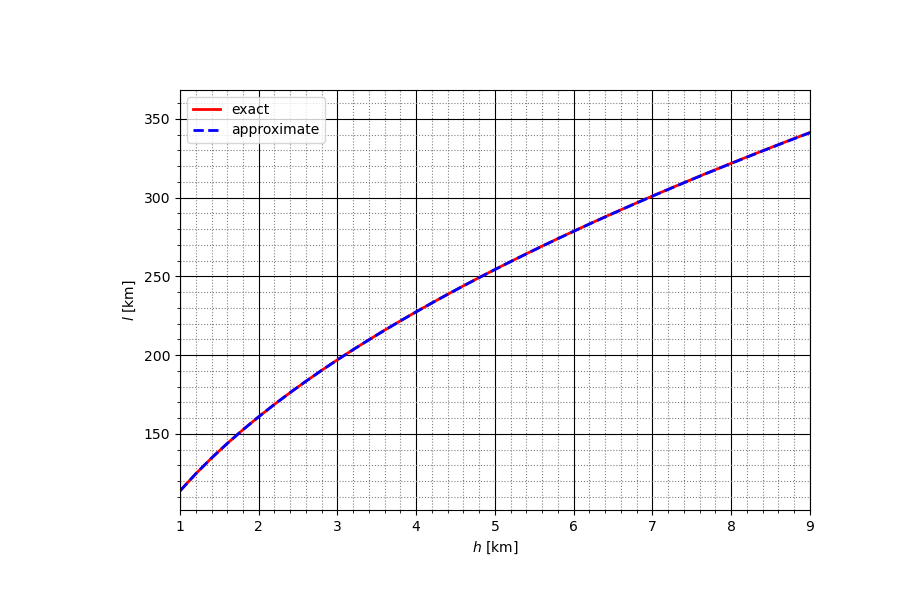
\includegraphics[width=130mm]{1.png}
 \caption{Зависимость дальности видимости $l$ от высоты горы $h$}
 \label{fig:2}
\end{figure}

\par
Выходит, что мы упростили выражение, не потеряв его сути. Этим и занимается математический анализ~\----~разрабатывает методы упрощения выражений, исследует малые и большие величины и как с ними стоит обращаться.

\subsection{Геометрическое доказательство теоремы Пифагора}
Выше была использована теорема Пифагора, важно помнить её простое геометрическое доказательство. Пускай есть прямоугольный треугольник с катетами $a$ и $b$ и гипотенузой $c$ (на чертежах ниже он выделен зелёным цветом). Рассмотрим квадрат со стороной $a+b$. Сперва разобьём его на два квадрата со стороной $a$ и со стороной $b$ и на 4 исходных треугольника таким образом, как показано на первом чертеже (см. рис. \ref{fig:3}.a). Получаем, что площадь большого квадрата есть сумма площадей квадратов поменьше ($a^2+b^2$) и четырёх площадей исходного треугольника.
\begin{figure}[h]
\begin{minipage}[h]{0.49\linewidth}
 \centering
 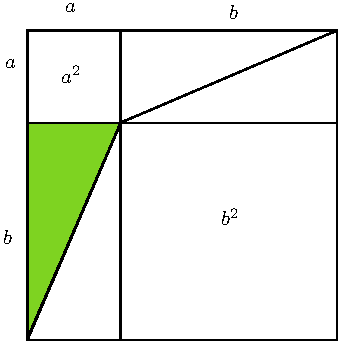
\includegraphics[scale = 1]{first21.pdf}
 \\
 a)
\end{minipage}
\hfill
\begin{minipage}[h]{0.49\linewidth}
 \centering
 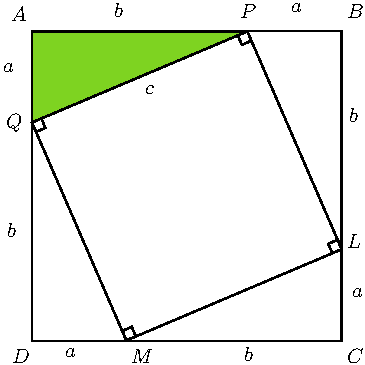
\includegraphics[scale = 1]{first22.pdf}
 \\
 b)
\end{minipage}
\caption{Чертежи к доказательству теоремы Пифагора. На чертеже a) представлено первое разбиение квадрата, на чертеже b)~\----~второе. Зелёным выделен исходный прямоугольный треугольник}
\label{fig:3}
\end{figure}
\par
Теперь разобьём квадрат так, как показано на втором чертеже (см. рис. \ref{fig:3}.b). То есть сначала строим четыре прямоугольных треугольника, как показано на чертеже. Затем замечаем, что получившийся из их гипотенуз ромб на самом деле является квадратом, ведь, например, развёрнутый угол $AQD$ состоит из углов $AQP$ и $MQD$, сумма которых равна девяноста градусам по свойству прямоугольного треугольника, а так же из угла $PQM$, которому ничего не остаётся, кроме как быть прямым (аналогичные рассуждения справедливы для каждого из углов четырёхугольника $QPLM$). То есть получилось, что площадь большого квадрата есть сумма площадей четырёх прямоугольных треугольников и площади квадрата со стороной $c$. Ясно, что площадь большого квадрата в том и другом случаях остаётся неизменной, тогда:
\begin{equation}
 a^2 + b^2 + 4S_\triangle=c^2+4S_\triangle
\end{equation}
Если сократить площади треугольников, то получим соотношение, называемое теоремой Пифагора:
\begin{equation}
 a^2 + b^2 =c^2
\end{equation}

\section{Вычисление массы Земли}
Рассмотрим несколько сюжетов, с помощью которых можно будет проиллюстрировать такие важные для математического анализа понятия, как производная и предел последовательности. 

\par
Начнём с рассмотрения примера о приближённом вычислении массы Земли. Пускай по некоторым физическим величинам производятся расчёты, но данные физические величины были измерены с ошибкой. Тогда как эта ошибка отразится на результате расчётов?

\subsection{Вычисление объёма Земли}
Обозначим за $R$ \emph{измеренное значение радиуса Земли}. Из\--за наличия ошибки измерений можно утверждать, что \emph{фактический радиус Земли} есть $R+\Delta R$, где за $\Delta R$ обозначена \emph{ошибка измерений радиуса Земли}. Как же эта ошибка повлияет на вычисленный объём земного шара (Земля полагается шарообразной)? Из школьного курса стереометрии должна быть известна формула объёма шара:
\begin{equation}\label{eq:6}
 V = \dfrac43 \pi R^3
\end{equation}
Обозначим через $V$ измеренный объём земного шара (он вычисляется по измеренному радиусу). А фактический объём Земли обозначим через $V + \Delta V$, где  за $\Delta V$ обозначена \emph{ошибка вычислений объёма Земли}. Тогда по той же формуле объёма шара пишем:
\begin{equation}\label{eq:7}
 V + \Delta V = \dfrac43 \pi \qty(R + \Delta R)^3
\end{equation}
Отсюда требуется найти $\Delta V$. Если вычесть из уравнения (\ref{eq:7}) уравнение (\ref{eq:6}), то получим:
\begin{equation}
 \Delta V = \dfrac43 \pi \qty(\qty(R + \Delta R)^3 - R^3)=\dfrac43 \pi \qty(3R^2\Delta R + 3R \Delta R^2 + \Delta R^3) = 4 \pi R^2\Delta R \qty( 1 + \dfrac{\Delta R}{R} +\dfrac{1}{3} \qty[\dfrac{\Delta  R}{R}]^2 )
\end{equation}
В итоговом виде равенства можно какими-то слагаемыми пренебречь. Например, измерили мы радиус Земли с точностью $1\%$, тогда в большой скобке стоит сумма трёх величин:
\begin{equation}
 1 + \dfrac{1}{100} + \dfrac{1}{3}\dfrac{1}{10000}
\end{equation}
Видно, что второе и третье слагаемые гораздо меньше первого, поэтому ими можно пренебречь. Тогда можно приближенно записать:
\begin{equation}\label{eq:10}
 \Delta V \approx 4 \pi R^2\Delta R
\end{equation}
Эта формула имеет простой геометрический смысл (см. рис. \ref{fig:4}). Синим обозначен земной шар в представлении тех, кто измерял его радиус, жёлтой штриховкой обозначен тонкий шаровой слой~\----~отличие измеренного земного шара от фактического. Объём этого шарового слоя обозначается за $\Delta V$. Если ошибка измерений радиуса мала, то площадь шарового слоя приближённо можно вычислить как объём прямоугольного параллелепипеда с площадью основания, равной площади сферы $4 \pi R^2$, и высотой $\Delta R$. Тогда и получаем формулу (\ref{eq:10}).
\begin{figure}[h]
 \centering
 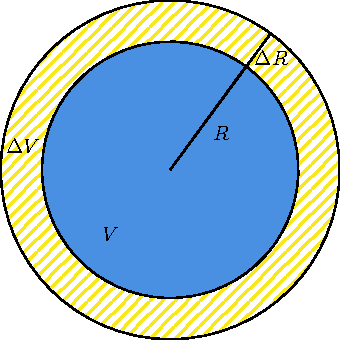
\includegraphics[scale = 0.8]{first3.pdf}
 \caption{Геометрическая аналогия к задаче об объёме Земли}
 \label{fig:4}
\end{figure}

\subsection{Завершение вычисления массы Земли}
Для того, чтобы определить массу планеты, нужно умножить среднюю плотность планеты на её объём. С последним мы уже разобрались. Средняя плотность Земли может быть измерена в ходе специальных экспериментов. Пускай через $\rho$ обозначено \emph{измеренное значение средней плотности Земли}, через $\rho + \Delta \rho$ обозначим \emph{фактическое значение средней плотности Земли}, где $\Delta \rho$~\----~\emph{ошибка измерения}. Тогда \emph{измеренная масса} $M$ будет равна:
\begin{equation}
 M = \rho V
\end{equation}
\emph{Фактическая масса} $M + \Delta M$ будет вычисляться по формуле:
\begin{equation}
 M + \Delta M = \qty(\rho + \Delta \rho) \qty(V + \Delta V)
\end{equation}
Тогда ошибка вычисления массы Земли будет:
\begin{equation}
 \Delta M = \Delta \rho \Delta V + \Delta \rho V + \rho \Delta V 
\end{equation}
Первое слагаемое является малым по сравнению с остальными, им можно пренебречь. Можно показать малость данного слагаемого геометрической аналогией (см. рис. \ref{fig:5}). Рассмотрим прямоугольник со сторонами $V$ и $\rho$. Его площадь будет равна измеренной массе Земли $M$. Тогда ошибки измерений можно представить как маленькие добавки к сторонам прямоугольника. Добавка к площади прямоугольника разбивается на три, площадь самого малого из добавочных прямоугольников соответствует слагаемому $\Delta \rho \Delta V$. Это показывает разумность пренебрежения им. Таким образом мы получаем:
\begin{equation}\label{eq:14}
 \Delta M \approx \Delta \rho V + \rho \Delta V 
\end{equation}
\begin{figure}[h]
 \centering
 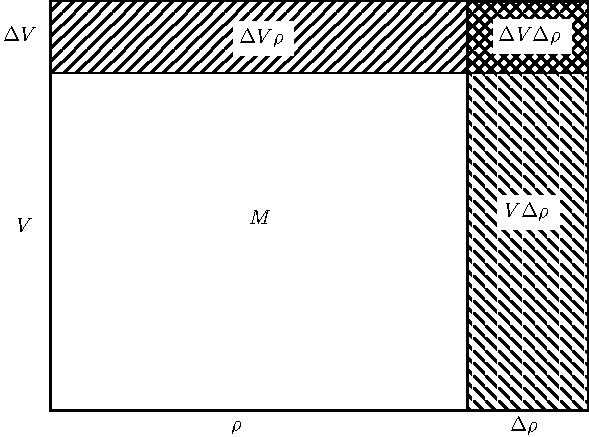
\includegraphics[scale = 0.8]{first4.pdf}
 \caption{Геометрическая аналогия к задаче о массе Земли}
 \label{fig:5}
\end{figure}

\subsection{Комментарии о значении полученных результатов}
Теперь приведём несколько комментарием о значениях этих формул для понимания математического анализа. Первая приближённая формула (\ref{eq:10}) для ошибки вычисления объёма земного шара представляет собой частный случай \emph{формулы производной от степенной функции}. Чтобы не давать строгих определений, запишем общую формулу в виде приближённого равенства:
\begin{equation}
 \Delta\qty(x^n) \approx n x^{n-1} \Delta x
\end{equation}
Она читается: <<Приращение функции $x^n$ есть произведение $nx^{n-1}$ на приращение $x$>>. В нашем случае $n=3$ и добавлен несущественный множитель $4\pi$.
\par
Вторая приближенная формула (\ref{eq:14}) есть не что иное, как \emph{правило дифференцирования произведения}. То есть приращение произведения двух величин есть сумма двух слагаемых: произведения приращения первой величины на вторую и произведения приращения второй величины на первую.
\par
Попробуем то же самое записать в терминах относительной погрешности. Относительная погрешность есть отношение абсолютной погрешности к измеренной величине. Например, относительная погрешность измерения радиуса:
\begin{equation}
 \varepsilon_R = \dfrac{\Delta R}{R}
\end{equation}
Для объёма получаем:
\begin{equation}
 \varepsilon_V = \dfrac{\Delta V}{V} = 3 \dfrac{\Delta R}{R} = 3 \varepsilon_R
\end{equation}
Для массы относительная погрешность будет:
\begin{equation}
 \varepsilon_M = \dfrac{\Delta M}{M} = \dfrac{\Delta \rho}{\rho} + \dfrac{\Delta V}{V}
\end{equation}
То есть относительная погрешность произведения двух величин равна сумме их относительных погрешностей.

\subsection{Немного цифр}
Рассмотрим численные значения физических величин, чтобы лучше понимать, о чём шла речь ранее. Радиус Земли можно оценить, как:
\begin{equation}
 R = 6.4 \vdot 10^6 \text{м} \pm 1\%
\end{equation}
То есть относительная погрешность измерения радиуса Земли составляет $1\%$.
Для плотности Земли имеем:
\begin{equation}
 \rho = 5.5 \tfrac{\text{т}}{\text{м}^3} \pm 1\%
\end{equation}
Тогда для объёма Земли получаем:
\begin{equation}
 V = 1.1\vdot10^{21}\text{м}^3 \pm 3\%
\end{equation}
Для массы Земли справедлив следующий ответ:
\begin{equation}
 V = 6.05\vdot10^{21}\text{т} \pm 4\%
\end{equation}



\end{document}
